\chapter{Overview of the Work}
This thesis introduces a pipeline for automating aspects of Linear B translation by combining probabilistic cognate matching, lightweight linguistic classifiers, and a prompted post-processing step.
The main components of the pipeline are:
\begin{enumerate}
    \item A cognate matching model, following Jiaming Luo \cite{luo}.
    \item Auxiliary classifiers that inform and constrain the decipherment: part of speech detection, noun type classification, and inflection detection.
    \item A prompt-engineering post-processor that proposes an Ancient Greek reconstruction and produces an English translation.
\end{enumerate}

\section{Chapters Overview}
Chapter \ref{chap:history} introduces the historical context of Aegean societies and their writing systems. Both Linear A and Linear B are outlined, together with the main stages of the Linear B decipherment.

Chapter \ref{chap:cognates} develops cognate matching, a core ingredient in computational decipherment. We formalize cognates and discuss matching principles grounded in proto-root similarity and phonological/morphological regularities.

Chapter \ref{chap:classifiers} presents the auxiliary tasks devised for this work and their models (part of speech detection, noun type classification, and inflection detection) together with the feature representations, training setup, and evaluation.

Chapter \ref{chap:pipeline} describes the full translation pipeline, explaining how to combine the cognate matching outputs and auxiliary predictions into a structured prompt for a large language model (LLM). The prompt design and the LLM's performance are discussed in detail.

Chapter \ref{chap:conclusion} summarizes the results of this work, discusses its limitations, and outlines possible directions for future research.

\section{Data Collection}
The data used in this work has been collected separately for Linear A, Linear B, and Ancient Greek.

\subsection{Linear A Fragments}
The Linear A fragments were collected from the corpora available at \url{https://sigla.phis.me} via web scraping.
Together with the fragments, site and document-level metadata were organized into a CSV with the following columns.

\paragraph{Field descriptions.}
\begin{itemize}
    \item \textbf{Site}: Archaeological site name (e.g., Arkhanes, Haghia Triada).
    \item \textbf{Number of Documents}: Total number of documents from that site in the  SigLA corpus (site-level count; repeated on each row for the site).
    \item \textbf{Document Name}: Canonical document identifier used by  SigLA (e.g., HT 117a, ARKH 1b); side labels a/b denote tablet faces.
    \item \textbf{Link}: Canonical URL to the  SigLA document page.
    \item \textbf{Type}: Document class (e.g., Tablet, Roundel).
    \item \textbf{Number of Signs}: Count of sign impressions recorded for the document (integer).
    \item \textbf{Number of Words}: Count of word tokens as segmented in the source (integer; can be 0 when only non-lexical marks are present).
    \item \textbf{Location}: Findspot within (or coincident with) the site when available; otherwise repeats the site name.
    \item \textbf{Period}: Archaeological period shorthand as in  SigLA (e.g., LM I, LM IB).
    \item \textbf{Motif}: Iconographic motif when applicable (common on roundels/seals; often empty for tablets), e.g., bull.
    \item \textbf{Width (cm)}: Maximum preserved width in centimetres (cm).
    \item \textbf{Height (cm)}: Maximum preserved height in centimetres (cm).
    \item \textbf{Depth (cm)}: Thickness in centimetres (cm).
\end{itemize}

\noindent\emph{Notes.} Missing values are left empty as in the source. Dimensions refer to the preserved object and follow  SigLA's measurements (decimal separator ".").

SigLA provides two parallel segmentations of each document: (i) a sign-by-sign view and (ii) a word/sequence view. The word view is not fully comprehensive: some isolated symbols are omitted and therefore never appear in the "words" export. For this reason, I keep the original sign segmentation as the authoritative layer, and use the word/sequence file to reconstruct identified sequences.

\paragraph{Signs CSV (per-sign records).}
Additional columns:

\begin{itemize}
  \item \textbf{Sign Number}: Running index of the sign within the document (starts at 1).
  \item \textbf{Sign}:  SigLA code of the sign (e.g., \texttt{ta}, \texttt{*118}, \texttt{AB16}, \texttt{[?]}).
  \item \textbf{Function}: Category of the sign (e.g., Syllabogram, Logogram) as given by  SigLA.
\end{itemize}

\paragraph{Words/Sequences CSV (per-word records).}
Additional columns:

\begin{itemize}
  \item \textbf{Sequence Number}: Running index of the sequence within the document (starts at 1).
  \item \textbf{Sequence}: Hyphen-separated syllabogram string exactly as in  SigLA (e.g., \texttt{a-su-mi-*118}).
  \item \textbf{Complete}: Boolean flag from  SigLA indicating whether the token is complete (True) or fragmentary/uncertain (False).
  \item \textbf{Length}: Number of syllabograms in the sequence (hyphen token count).
\end{itemize}

The algorithm used to reconstruct full documents, by aligning the sign and word sequences, is described in Algorithm \ref{alg:la-reconstruct}.

\begin{algorithm}[H]
\DontPrintSemicolon
\SetAlgoNoLine

\SetKwInOut{Input}{Input}
\SetKwInOut{Output}{Output}

\Input{For each document $d$: ordered $\mathrm{SIGN\_STREAM}_d = (s_1,\dots,s_m)$ by sign\_number; ordered $\mathrm{WORDS}_d = (w_1,\dots,w_n)$ where $w_j = (w_{j,1},\dots,w_{j,k_j})$ are syllables split by ``-''.}
\Output{$\mathrm{docs}[d]$: space-separated token stream.}

\ForEach{document $d$}{
  $\mathrm{out} \gets \langle\,\rangle$;\quad $\mathrm{buf} \gets \langle\,\rangle$;\quad $j \gets 1$;\quad $i \gets 1$\;

  \For{$t \gets 1$ \KwTo $m$}{
    \eIf{$j \le n \ \wedge\ s_t = w_{j,i}$}{
      \eIf{$i = k_j$}{ % full word
        emit $w_j$ as a complete word (syllables joined by "-") into $\mathrm{out}$;\quad
        $\mathrm{buf} \gets \langle\,\rangle$;\quad $i \gets 1$;\quad $j \gets \min(j{+}1,\,n)$\;
      }{
        append $s_t$ to $\mathrm{buf}$;\quad $i \gets i{+}1$\;
      }
    }{
      \If{$\mathrm{buf} \neq \langle\,\rangle$}{emit elements of $\mathrm{buf}$ into $\mathrm{out}$ in order;\quad $\mathrm{buf} \gets \langle\,\rangle$;\quad $i \gets 1$}
      emit $s_t$ into $\mathrm{out}$\;
    }
  }

  \If{$\mathrm{buf} \neq \langle\,\rangle$}{emit elements of $\mathrm{buf}$ into $\mathrm{out}$ in order}

  $\mathrm{docs}[d] \gets$ concatenate tokens of $\mathrm{out}$ with a single space
}

\caption{Align sequences $w_j$ to stream $(s_t)$: on full match emit $w_j$; else emit unmatched syllabograms.}
\label{alg:la-reconstruct}
\end{algorithm}

\subsection{Linear B Documents}
The Linear B corpus was similarly webscraped from the LiBER (Linear B Electronic Resources) archive \url{https://liber.cnr.it/tablet/list}.
However, the LiBER archive provides only a word-level segmentation, with no underlying sign-by-sign layer.
Because many Linear B documents are fragmented and carry annotations and uncertain signs, the data required cleaning to standardize the representation of extracted syllabograms.
The cleaned data was organized into three CSV files, as in the previous case.

The data of Linear B documents was organized as follows: the first CSV contains the document-level information, using the following fields.

\paragraph{Signs CSV (per-sign records).}Part of Speech
Additional columns:
\begin{itemize}
  \item \textbf{Sign Number}: Position of the sign within the document (starts at 1).
  \item \textbf{Sign}: Cleaned Linear B symbol (syllabogram / logogram / numeral / uncertain), e.g., pu, \texttt{M}, \texttt{1}, \texttt{[?]}.
\end{itemize}

\paragraph{Words/Sequences CSV (per-word records).}
Additional columns:
\begin{itemize}
  \item \textbf{Sequence Number}: Position of the word within the document (starts at 1).
  \item \textbf{Sequence}: Hyphen-separated cleaned symbols, e.g., \texttt{e-ri-sa-ta}, \texttt{M}, \texttt{1}.
  \item \textbf{Complete}: True/False flag from LiBER indicating whether the token is complete.
  \item \textbf{Length}: Number of syllabograms in the sequence.
\end{itemize}
The full webscraping and processing of Linear B data is detailed in Figure \ref{fig:webscrape-lb}.

\begin{figure}[H]
    \begin{adjustbox}{center}
        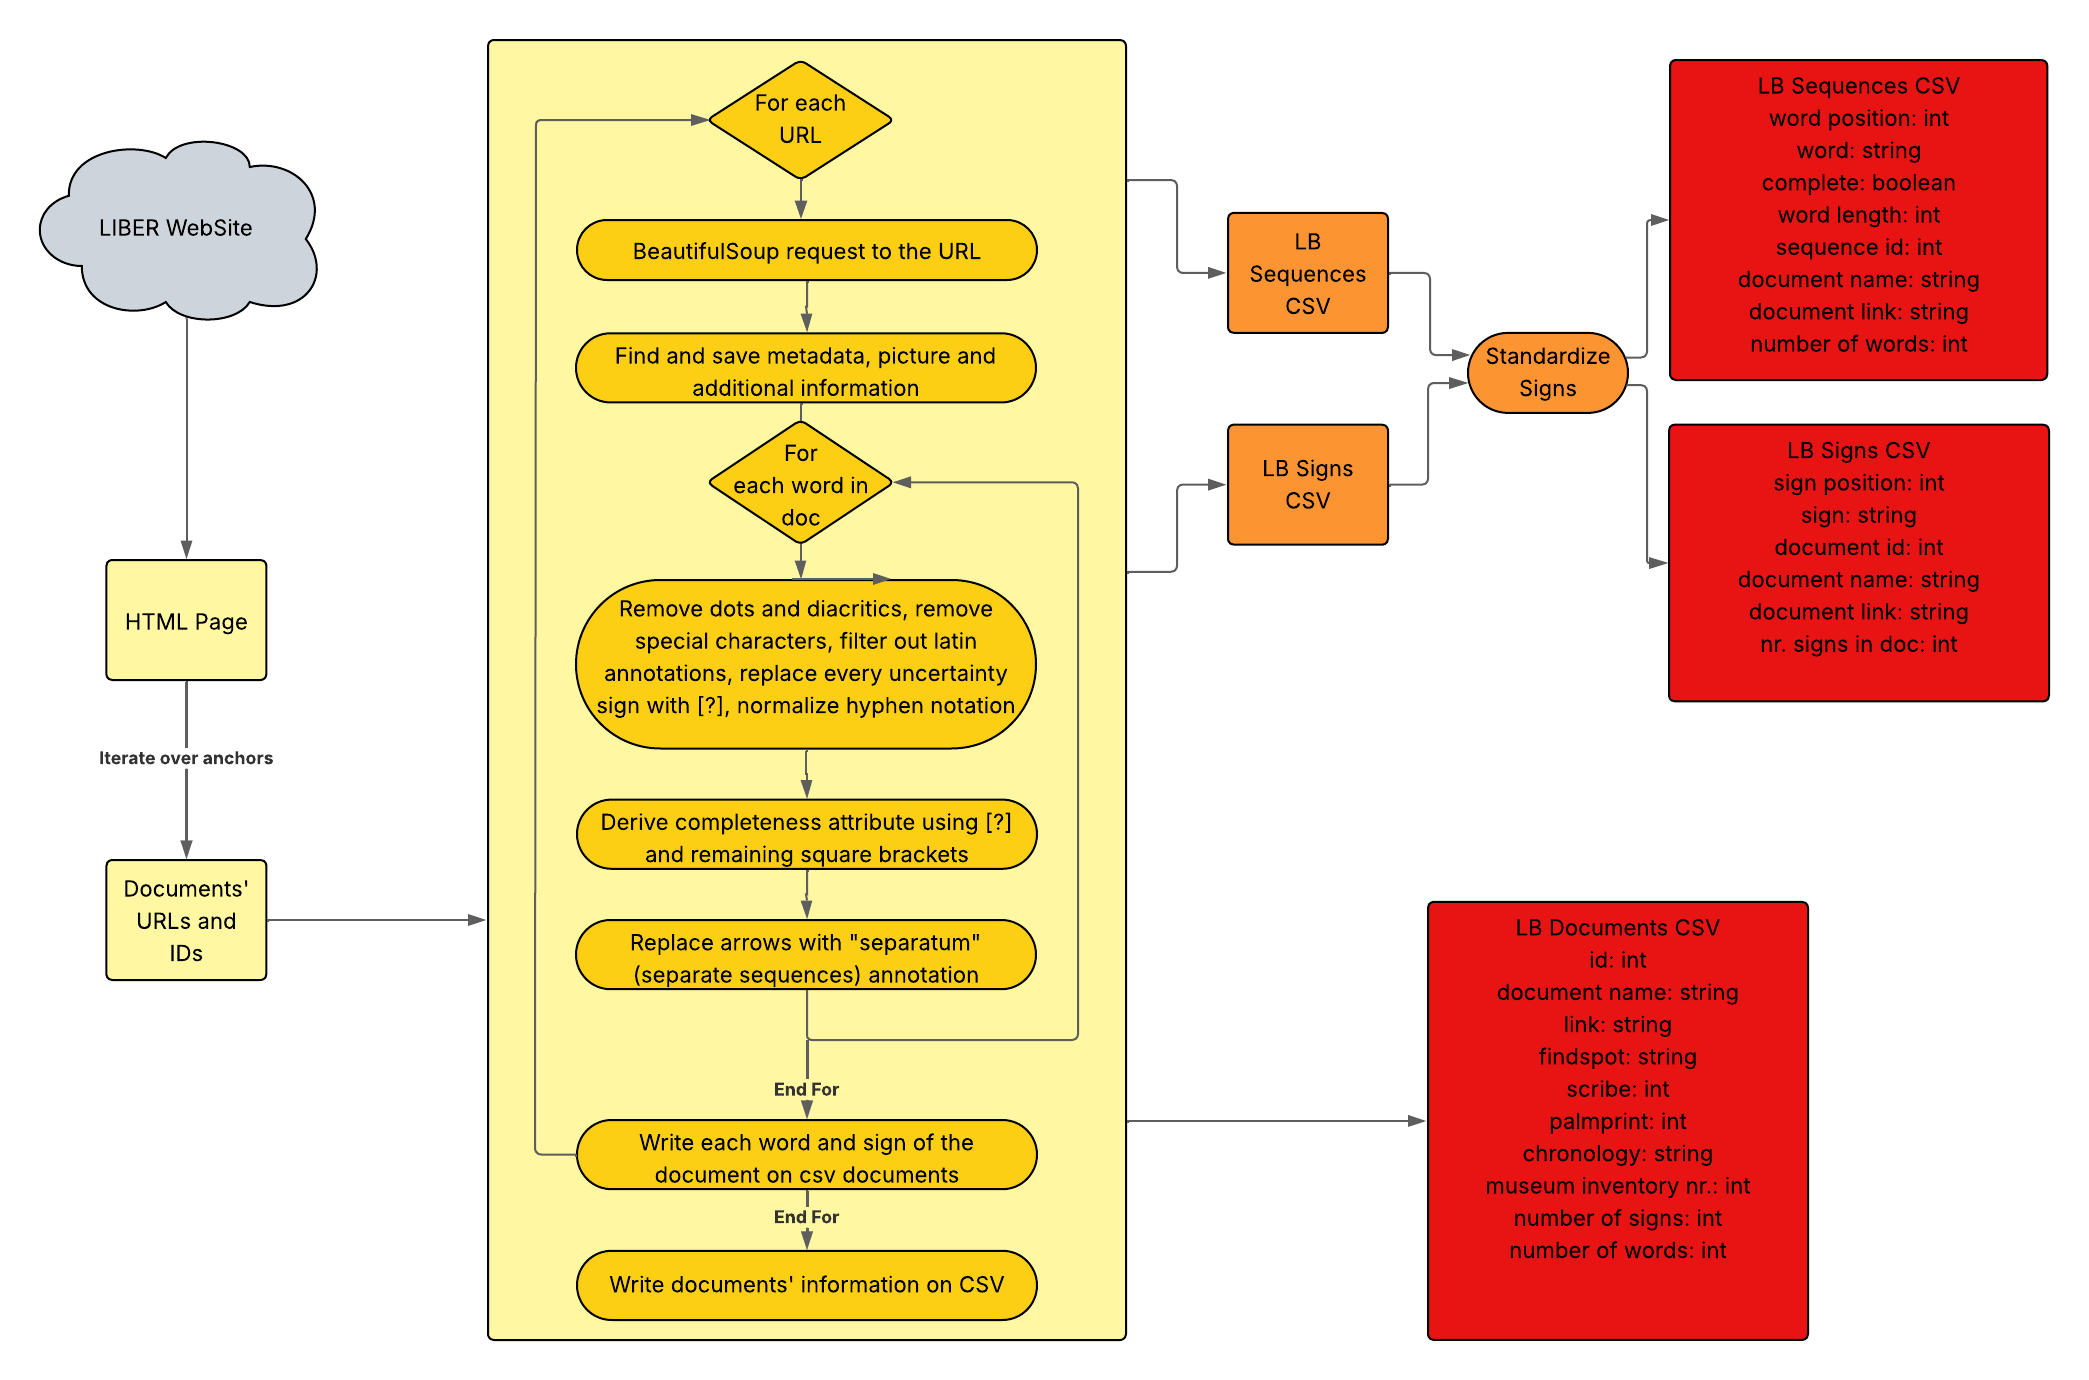
\includegraphics[width=1.1\textwidth]{images/webscrape_linb.png}
    \end{adjustbox}
    \caption{Webscraping and processing of Linear B data from the LiBER archive.}
    \label{fig:webscrape-lb}
\end{figure}

\subsection{Ancient Greek}
For Ancient Greek we required a broad lexicon, preferably skewed toward earlier forms that preserve Mycenaean reflexes more than later Classical usage.
To that end, the Homeric epics (the Iliad and the Odyssey) were collected and preprocessed to a normalized orthography, described in Section \ref{sec:datasets}.

The resulting high-coverage type list serves the brute-force cognate matching stage (Section \ref{sec:bruteforce-cognates}), where the entire Linear B corpus is compared against normalized Homeric forms to surface plausible cognate candidates.

\section{Related Work}
The work presented in this thesis builds upon and extends prior research in historical linguistics, computational decipherment, and natural language processing.

For the historical and linguistic background of Aegean scripts, I relied on foundational texts, such as Minoan Civilization by Spyros Alexiou \cite{alexiou-ch2}, Aegean Linear Script(s) by Ester Salgarella \cite{salg-ch1}, and The Decipherment of Linear B by John Chadwick \cite{chad-ch2}.

In the realm of computational decipherment, the most relevant prior work consisted of contributions on the text infilling task by Katerina Papavassileiou \cite{brnn-paper} and the cognate matching task by Jiaming Luo \cite{luo}.  
Notably, in both cases the models used to encode Linear B sequences are based on bidirectional recurrent neural networks (BRNNs), which are also used in this work.  
For the text infilling task, I also assessed the effectiveness of transformer-based architectures, noting a significant drop in performance compared to RNNs, mostly due to the scarcity of training data. 

Lastly, the prompt-engineering approach to translation and reconstruction is inspired by the advantages of large language models and their demonstrated ability to understand and translate Ancient Greek.  
By supplying the information that is strictly necessary for translation and reconstruction, the Linear B corpus can be automatically translated into English.

\subsection{Cognate Matching and Manual Decipherment}
Cognate matching has been used in several prior works to support the decipherment of ancient scripts.  
Ventris and Chadwick themselves relied on simple cognate identification at the start of their decipherment of Linear B.  
Automating cognate detection is a crucial step toward scaling decipherment efforts to larger corpora and more complex scripts.  
Luo proposed a language-agnostic neural model for cognate matching, which I tested and extended in this thesis (Section \ref{sec:generative-framework}).

The model's output was used to generate a list of candidate cognate pairs, which were provided as input to an LLM.  
Alongside these, I supplied additional linguistic information useful for grammatical, logical, and syntactical analysis.  
The LLM was then prompted to produce an Ancient Greek reconstruction and translate it into English, using structured processing instructions, typical of manual decipherment, and a few examples.  
The steps of this process are described in detail in Section \ref{sec:final-prompt}.

